\documentclass[serif ,mathserif, 8pt]{beamer}
\usepackage{pxfonts}
%\usepackage{eulervm}


%%-------------------------
%  ---- BEAMER THEME ---
%%--------------------------
\usetheme{AnnArbor}
\usecolortheme{crane}
\setbeamercovered{transparent}
%\setbeamercolor{section in head/foot}{use=structure,bg=structure.fg!55!bg}
\setbeamerfont{frametitle}{series=\bfseries} % Frame titles should be bold
\useinnertheme[shadow=true]{rounded}
\useoutertheme[subsection=true]{smoothbars}%Beamer Outer Theme-circles on top
%\useinnertheme{circles} %rectangle bullet points instead of circle ones
%\mode<presentation>
%\newcommand*\oldmacro{}%
%\let\oldmacro\insertshorttitle%
%\renewcommand*\insertshorttitle{%
%  \oldmacro\hfill%
%  \insertframenumber\,}%/\,\inserttotalframenumber
%\setbeamertemplate{footline}[frame number]
%%-------------------------------------------------------------------

\usepackage[utf8]{inputenc}
\usepackage[english]{babel}
\usepackage[T1]{fontenc}
\usepackage{amsmath}
\usepackage{graphicx}
\usepackage{url}
\usepackage{xcolor}
\usepackage{hyperref}
\hypersetup{
	colorlinks = true, linkcolor=blue!45!black, citecolor=black, anchorcolor=green,
	pdfstartview=FitH, pdffitwindow=true, pdfmenubar=true,
	pdfcreator=PDFLaTeX, pdfproducer=PDFLaTeX, 
	pageanchor=true, backref,
	hyperindex=true}
\usepackage{multimedia,animate}
%\usepackage{xmpmulti}
\usepackage{media9}
\usepackage{ragged2e}
\usepackage{wasysym}

\author{\textbf{H. Ghalila, A. Ammar*, Y. Majdi, S. Lahmar, Z Dhaoudi, M. Zghal, Zohra Ben Lakhdar, V. Lakshminarayanan*}}
\title{Hands-on experimental and computer laboratory in optics}
\subtitle{The Young Double Slit Experiment}
\setbeamercovered{transparent} 
%\setbeamertemplate{navigation symbols}{} 
%%%%%%%%%%%%%%%%%%%%%%%%%%%%%%%%  L O G O   %%%%%%%%%%%%%%%%%%%%%%%%%%%%%%%
%\logo{%
%    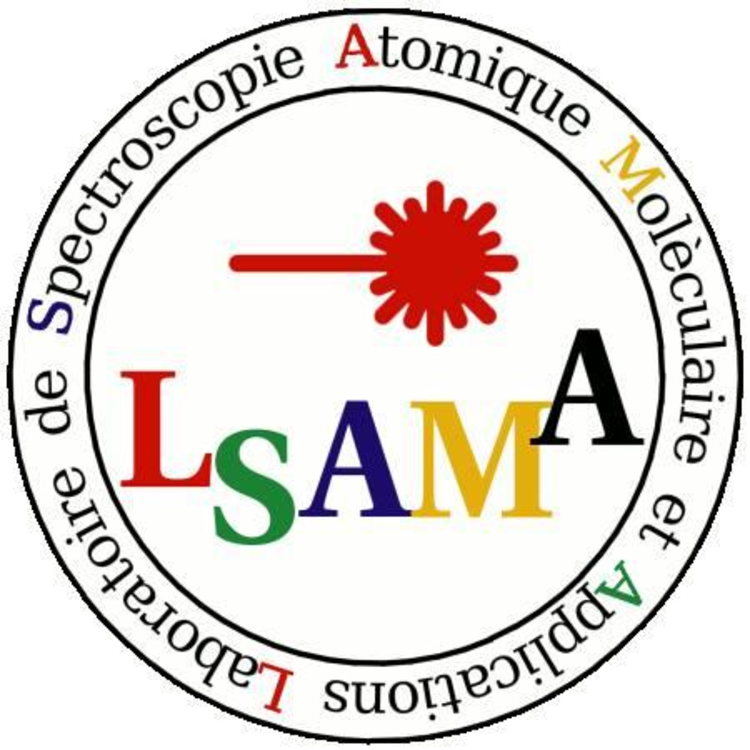
\includegraphics[width=1cm,height=0.8cm,keepaspectratio]{images/logoLSAMA}%
   % \includegraphics[width=1cm,height=1cm,keepaspectratio]{images/logoH}~%
    %\includegraphics[width=1cm,height=1cm,keepaspectratio]{logo3}%
%}

\institute[LSAMA Lab \& Optical Society of Tunisia]{
\includegraphics[width=3cm]{images/STO_logo} 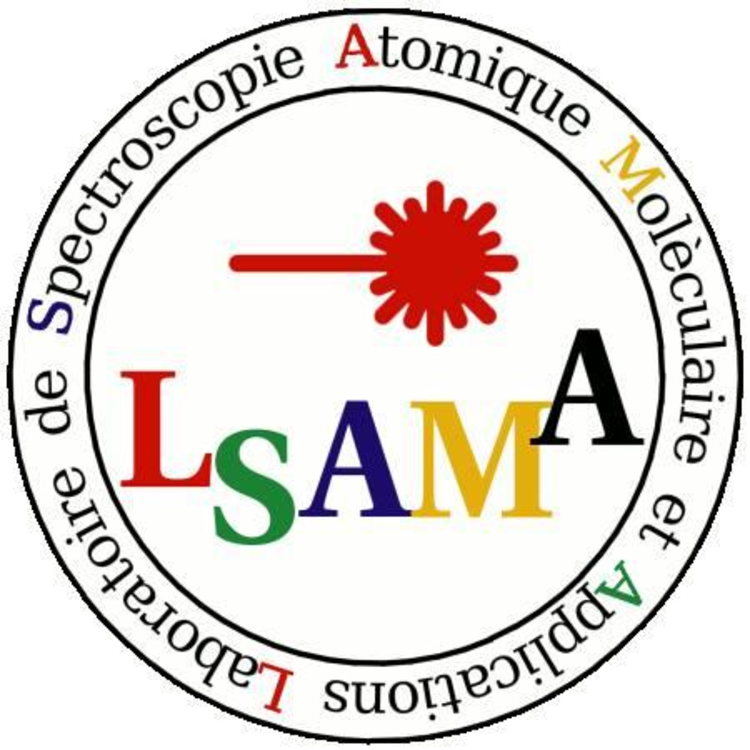
\includegraphics[width=1.5cm]{images/logoLSAMA} \\
Optical Society of Tunisia \& LSAMA Lab, Faculty of Sciences of Tunis}
%%%%%%%%%%%%%%%%%%%%%%%%%%%%%%%%%%%%%%%%%%%%%%%%%%%%%%%%%%%%%%%%%%%%
%\institute{} 
\date{\today} 
%\subject{} 
\usepackage[style=verbose-note,autocite=footnote,abbreviate=true]{biblatex}
%\usepackage{filecontents}

\begin{document}
\begin{frame}
\titlepage
\end{frame}
\begin{frame}{Teaching has not changed over the centuries!}
		\centering
		\begin{figure}
			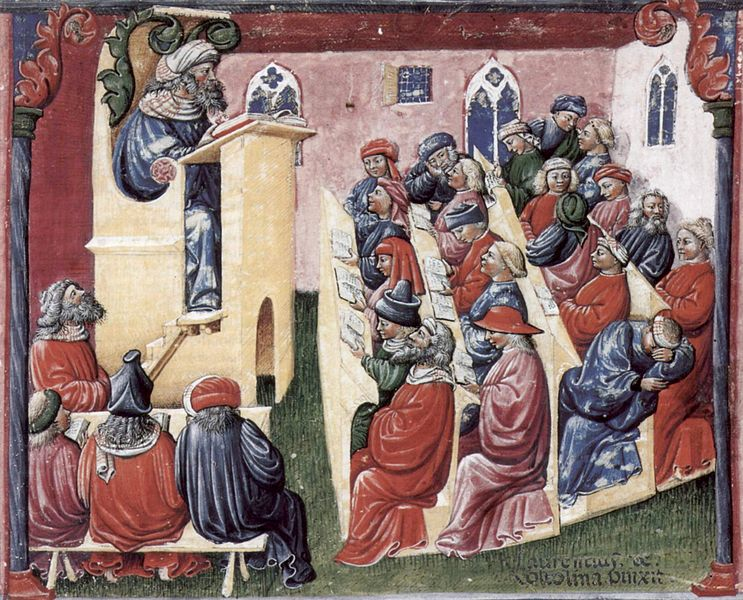
\includegraphics[width=.65\linewidth]{images/Laurentius_de_Voltolina_001}
			\caption{Henry of Germany lecturing at the University of Bologna. Painting by Laurentius de Voltolina (1350).}
		\end{figure}
		
\end{frame}

\begin{frame}{Active learning cycle}
	\begin{columns}[c]
		\begin{column}{0.6\textwidth}
				Teacher has to change the classical and usually passive way of teaching to one favoring Predictions, Observations, Discussions and Syntheses (PODS).
				
				
		\begin{exampleblock}{Learning through experimentation}
			Active Learning in Optics and Photonics (ALOP) UNESCO’s programme is the best example for this concept that provide a set of experiments to understand optics and photonics.
		\end{exampleblock}
		\begin{alertblock}{Learning through simulation}
			ALOP does not contain computations or simulations. “Active learning” and “Optics simulations” together may be joined as “Active Learning in Simulating Optics” (ALSO).\\
			Our goal is to encourage teachers and students to take an active part in developing their own codes as they design individual own experiments.\\
			
		\end{alertblock}
		\end{column}
		\begin{column}{0.4\textwidth}
			\begin{figure}
				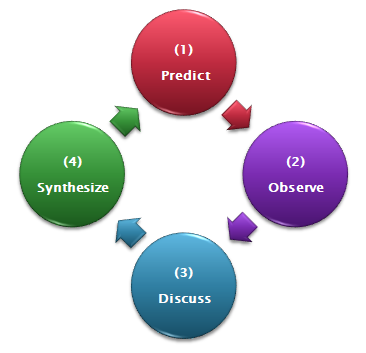
\includegraphics[width=\linewidth]{images/alop_cycle}
				\caption{ALOP learning cycle.}
			\end{figure}
		\end{column}
	\end{columns}
		
\end{frame}

\begin{frame}{Active Learning in Simulating Optics (ALSO)}

\begin{block}{Some of the criteria for a good computer simulation for classroom use}
	Some of the criteria that are relevant for learning via simulation include:
	\begin{itemize}
		\item The simulations should be true to life. That is, they should simulate the activity so well that there is little
		difference between the simulated environment and the real one, and the same kind of learning experience can
		take place.
		\item The simulations should be “hand-on,” involving the students so that the students become participants in the
		simulation activity. This implies that students interact with the simulation, for example, by changing parameters, changing lines in the code, discussing the simulated results, etc.
		\item Simulations should motivate learning. Student involvement in the activity should be such they are motivated to learn more about the activity or the subject matter.
		\item Simulations should be customizable to the students' needs. Students' developmental requirements should be
		taken in consideration while designing simulations specifically for them.
		\item Simulations are meant to supplement, not replace other teaching modes. Integrating simulations into the
		curriculum also ensures that connections to domain knowledge and real-world applications are made explicit.
		\item As with any instructional technology, computer simulations should be chosen to meet the teaching objectives
		and teach the content.
	\end{itemize}
\end{block}

\end{frame}

\begin{frame}{Optics simulation with Python}
\begin{columns}[c]
	\begin{column}{0.6\textwidth}
		\begin{block}{What is Python?}
			Python is a modern, general-purpose, object oriented, high-level programming language.
			\begin{itemize}
				\item \textbf{Clean and simple language:} Easy-to-read and intuitive code, easy-to-learn minimalistic syntax, maintainability scales well with size of projects.
				\item \textbf{Expressive language:} Fewer lines of code, fewer bugs, easier to maintain.
				\item \textbf{Powerful Python packages:} open source pre-built and tested scientific and
				analytic Python packages that include NumPy, Pandas, SciPy, Matplotlib...
				\item \textbf{An easy way to install Python and its packages:} Anaconda is a cross platform Python distribution and easy-to-install free package and environment manager.
			\end{itemize}
		\end{block}
		
	\end{column}
	
	\begin{column}{0.4\textwidth}
		\begin{figure}
			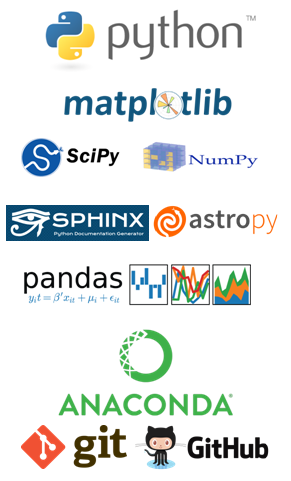
\includegraphics[width=.8\linewidth]{images/python}
		\end{figure}
	\end{column}
\end{columns}

\end{frame}

\begin{frame}{Example: The Young Double Slit Experiment}
	\begin{block}{ALOP, Zimbabwe, July 2018}
		\centering
		\begin{figure}
			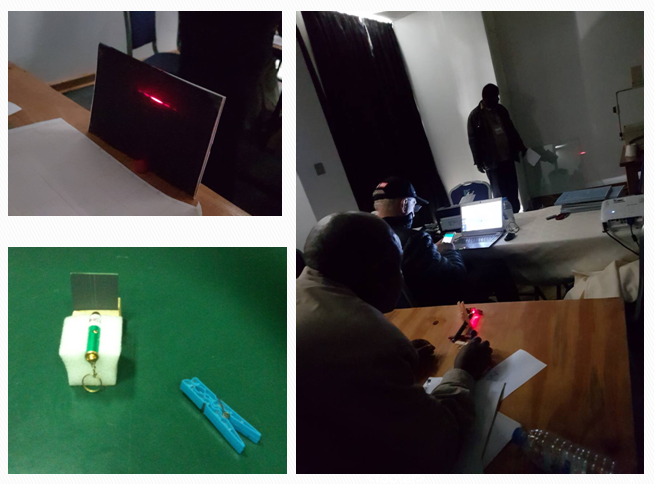
\includegraphics[width=.7\linewidth]{images/alop2018}
		\end{figure}
	\end{block}
\end{frame}
\begin{frame}{Observation}
	\centering
	\begin{figure}
		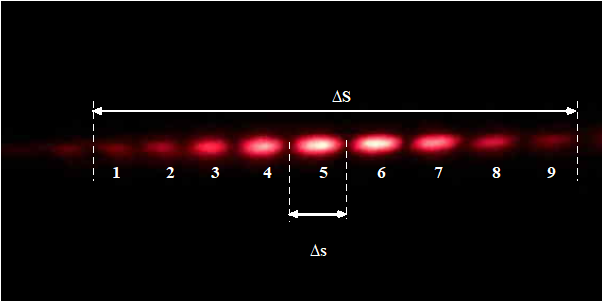
\includegraphics[width=.9\linewidth]{images/Image1}
		\caption{Measures of the size of the main central peak of diffraction $\Delta S$, the size of the small spot du to the interferences $\Delta s$ and enumeration of the number of interference peak inside the main peak of diffraction
		}
	\end{figure}

\end{frame}
\begin{frame}{Numerical modeling}
\begin{columns}[c]
	\begin{column}{0.35\textwidth}
		\begin{block}{Experiment}
			\begin{figure}
				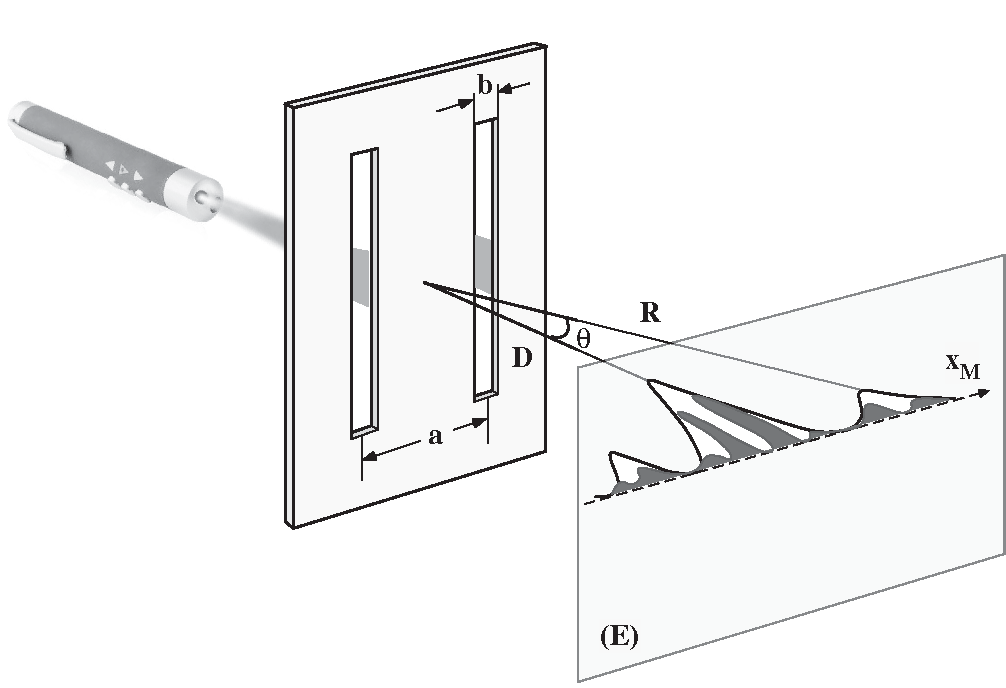
\includegraphics[width=\linewidth]{images/DoubleFente}
			\end{figure}
		\end{block}
		
	\end{column}
	
	\begin{column}{0.55\textwidth}
		\begin{block}{Model}
			\begin{figure}
				
				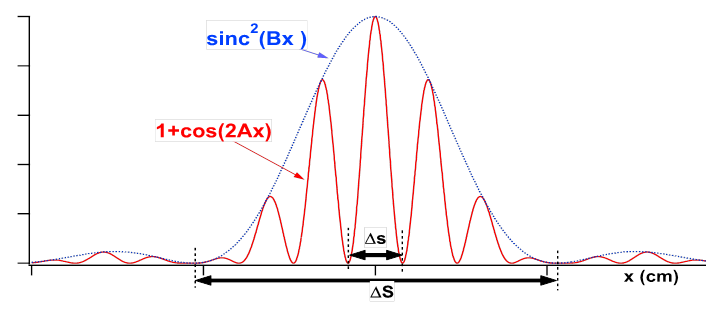
\includegraphics[width=\linewidth]{images/im2}
			\end{figure}
		\end{block}
			
	\end{column}
\end{columns}
	
\begin{block}{Analytical expression}
	\begin{equation*}
	I(x) = sinc^2 (Bx)[1+cos(2Ax)] \quad \quad where: \ A = \pi a /\lambda D \ and \ B = \pi b / \lambda D
	\end{equation*}
	$b$ stands for the width of the slits, $a$ represents the distance between slits, $D$ is the distance of the screen to the plan of the slits and $\lambda$ is the wavelength of the monochromatic incident light.\\
	The values of $\Delta S$ and $\Delta s$ are determined theoretically from $b$ and $a$ :\\
	\begin{center}
		$\Delta S=2\lambda D/b$	\quad and \quad $\Delta s=\lambda D/a$
	\end{center}

\end{block}


\end{frame}

\begin{frame}{Python application}
	\centering
	\animategraphics[loop,autoplay, controls,width=.95\linewidth]{2}{images/demo/out}{1}{118}\\
	Clone or download the code source from GitHub:\\
	\url{https://astrax.github.io/ETOP_2018/}	
\end{frame}

%\begin{frame}{Python application}
%	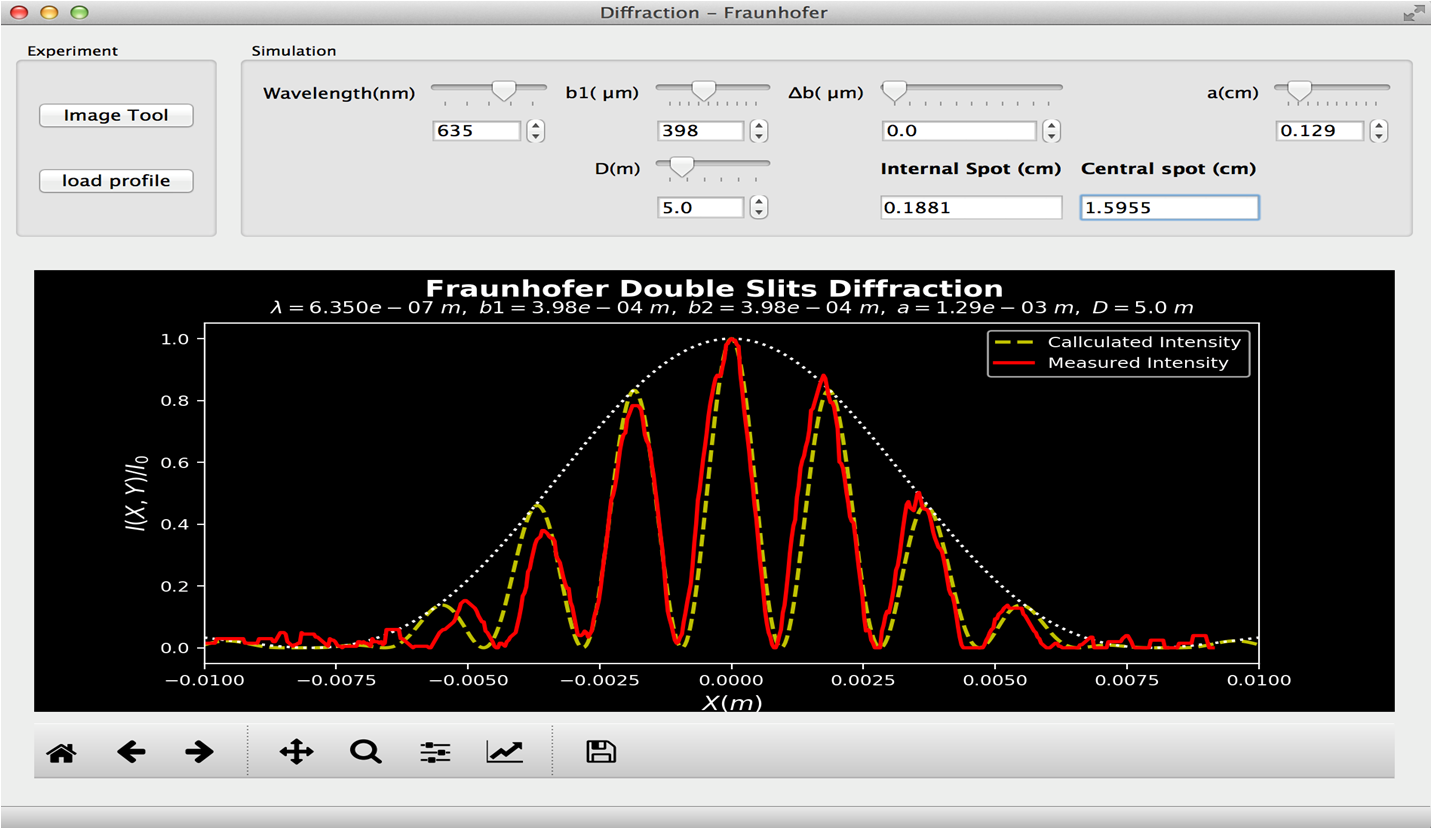
\includegraphics[width=\linewidth]{images/Image3}\\
%Clone or download the code source from GitHub:\\
%\url{https://github.com/astrax/ETOP_2018}
%\end{frame}

\begin{frame}{New published text book}
\begin{columns}[c]
	\begin{column}{0.6\textwidth}
		More than 50 programs and applications are free to download on the book's web page: \url{www.crcpress.com/9781498755047}
		
		\begin{figure}
			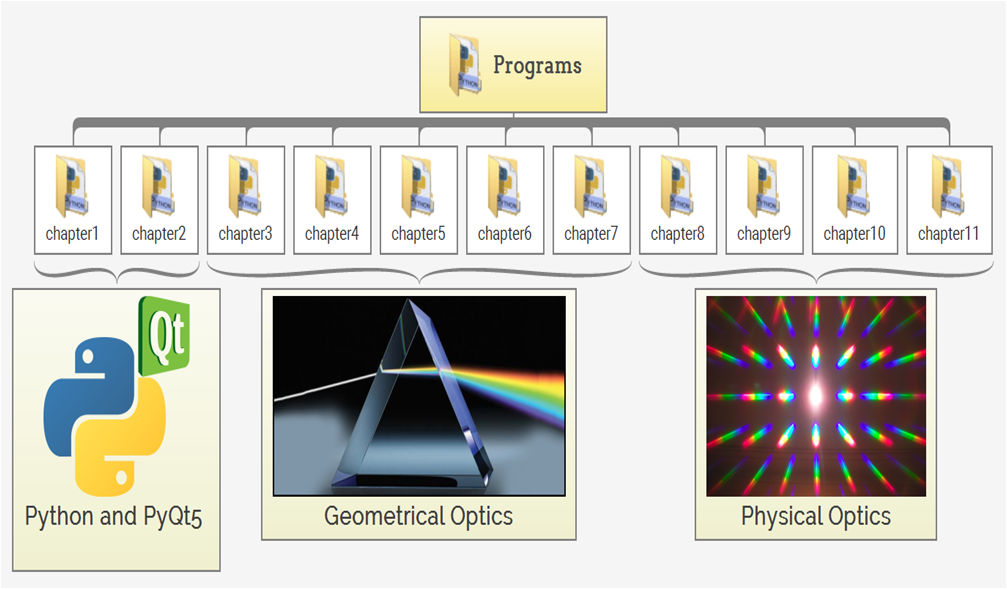
\includegraphics[width=\linewidth]{images/Image4}
			
		\end{figure}
		
		
	\end{column}
	\begin{column}{0.4\textwidth}
		\begin{figure}
			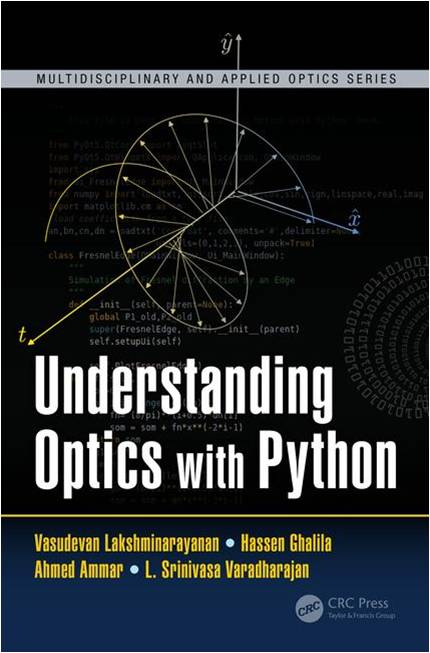
\includegraphics[width=\linewidth]{images/Image5}
			
		\end{figure}
	\end{column}
\end{columns}

\end{frame}

%\begin{frame}{Active Learning in Simulating Optics (ALSO)}
%It is essential for the student to learn the concepts behind the equations.
%\end{frame}

\begin{frame}
\centering
\huge \textbf{Thank you!}
\end{frame}

\end{document}
